\chapter{The RBMK-1000 Reactor}
\label{ch:rbmk}

To understand Chernobyl one must understand the machine. The RBMK-1000
(\emph{reaktor bolshoy moshchnosti kanalnyy}---high-power channel-type reactor) was
a uniquely Soviet design whose distinctive features---graphite moderation, water
cooling in individual pressure tubes, on-load refuelling, and a very large
core---combined to give it the destabilising characteristics that the accident
exposed. This chapter dissects the design with particular attention to the
features that bear on thermal stability: the positive void coefficient and the
flawed control-rod design.

\section{Design philosophy and layout}

The RBMK was conceived to produce both electricity and, in its lineage, plutonium,
and to use natural or low-enriched uranium with on-load refuelling and
domestically available technology. It dispensed with the massive single
pressure vessel of a Western PWR. Instead, the core was an enormous stack of
graphite blocks---about $12\unit{m}$ in diameter and $7\unit{m}$ tall, weighing
some $1700\unit{tonnes}$---penetrated by roughly $1660$ vertical
\textbf{pressure tubes} (fuel channels). Each channel held fuel assemblies of
slightly enriched ($\sim 2\%$) $\mathrm{UO_2}$ and carried boiling light water as
coolant. The water boiled in the channels (like a BWR), and the steam was
separated and sent to the turbines.

The decisive architectural fact is the \emph{separation of moderator and coolant}.
In a PWR or BWR the water is both moderator and coolant, so losing water loses
moderation. In the RBMK the \textbf{graphite} did the moderating, and the water was
mainly coolant---and, because water absorbs thermal neutrons, also a parasitic
absorber. This separation is the root of the positive void coefficient.

\section{The positive void coefficient}

Consider what happens when the cooling water in an RBMK channel boils more
vigorously, increasing the steam void fraction. Two effects compete, as in any
water reactor (Chapter~\ref{ch:feedback}): loss of moderation (tends to reduce
reactivity) and loss of neutron absorption (tends to increase it). In the RBMK the
graphite continues to moderate regardless of the water, so the loss-of-moderation
effect is weak; what dominates is the removal of the water \emph{absorber}.
Boiling the water therefore \emph{adds} reactivity:
\begin{equation}
\alpha_v = \frac{\partial \rho}{\partial \bar v} > 0,
\end{equation}
strongly positive. The magnitude depended on the core state---fuel burnup,
enrichment, and especially the number of control rods inserted and the operating
reactivity margin. In the configuration of the accident, the void coefficient was
large enough that the total power coefficient at low power was \emph{positive}: a
rise in power boiled more water, which raised reactivity, which raised power---a
self-amplifying loop with no prompt negative effect strong enough to counter it.

\begin{figure}[H]
\centering
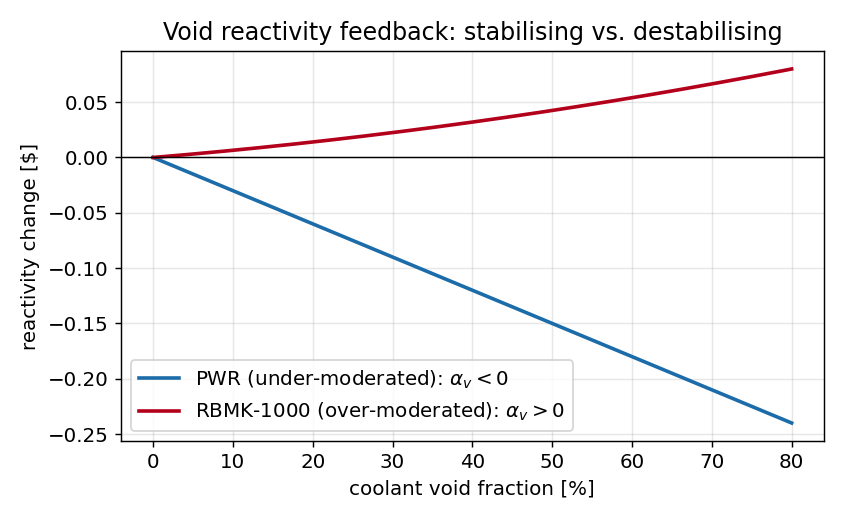
\includegraphics[width=0.74\linewidth]{figures/void.png}
\caption{The RBMK's over-moderated lattice gives a positive void coefficient
(rising curve): boiling adds reactivity, in contrast to the negative void
coefficient of an under-moderated PWR. This is the central design flaw behind
Chernobyl.}
\label{fig:void-rbmk}
\end{figure}

\section{The graphite moderator and the positive feedback chain}

The large graphite mass gave the RBMK a long prompt neutron lifetime and a great
deal of thermal inertia, which in some respects made the reactor sluggish and
seemingly forgiving. But the same graphite is what decoupled moderation from the
coolant and produced the positive void coefficient. Graphite also stores energy
(Wigner energy) and burns in air at high temperature---both relevant to the
accident's aftermath, when the exposed graphite caught fire and lofted fission
products for days. The design thus combined a destabilising neutronic
characteristic with a flammable moderator, a doubly unfortunate pairing.

\section{The fatal control-rod design}

The RBMK's most notorious flaw lay in its control rods. Each absorber rod was
fitted, on its lower end, with a \textbf{graphite ``displacer'' (follower)} about
$4.5\unit{m}$ long, separated from the boron-carbide absorber by a short column of
water. The purpose of the graphite tip was to keep water (an absorber) out of the
channel below a withdrawn rod, improving efficiency. The consequence was lethal.

When a rod was fully withdrawn, its graphite displacer sat in the central region
of the core and the lower portion of the channel was filled with water. As the rod
began to insert from the fully-withdrawn position, the leading element to enter the
core's lower region was not the boron absorber but the \emph{graphite displacer},
which \emph{displaced water} (an absorber) with \emph{graphite} (a moderator). The
immediate, local effect of beginning to insert the rod was therefore to
\emph{add} positive reactivity in the lower core---before the absorber section
arrived to add the intended negative reactivity. This is the \textbf{positive
scram effect}: pressing the emergency shutdown button could, for the first few
seconds and especially with an axially bottom-peaked flux, momentarily
\emph{increase} reactivity.

\begin{remark}[A known flaw, unaddressed]
The positive scram effect was not unknown. A similar control-rod-insertion power
spike had been observed at the Ignalina RBMK in 1983, and the phenomenon was
understood in principle. Yet the design was not corrected and operators were not
adequately warned. INSAG-7 later noted that there was a widespread belief that the
conditions under which the positive scram effect would matter ``would never
occur''---conditions that, in the event, ``appeared in almost every detail'' at
Chernobyl.
\end{remark}

\section{The operating reactivity margin}

Because the RBMK relied on a substantial number of inserted control rods to shape
its flux and maintain controllability, operating rules specified a minimum
\textbf{operating reactivity margin (ORM)}---expressed as an equivalent number of
fully-inserted control rods (nominally about $30$, with a hard floor of $15$). The
ORM was, in effect, the reactor's shutdown reserve and its guarantee of
controllability and acceptable feedback characteristics. Operating below the
minimum ORM was prohibited because it left too few absorbers to shut the reactor
down quickly and---crucially---worsened the void coefficient and the axial power
shape. On the night of the accident the ORM was driven far below the limit, to the
equivalent of perhaps six to eight rods, in the struggle against xenon poisoning.

\section{The instrumentation and protection gaps}

The RBMK's protection systems and instrumentation compounded the physical flaws.
The emergency shutdown was slow---full rod insertion took on the order of
$18\unit{s}$, an eternity for a prompt excursion. Key automatic protection
trips had been disabled to permit the test. The control system did not enforce the
ORM limit automatically. And the operators' training and documentation did not
convey the true severity of the low-power, low-ORM regime. The machine's safety
thus depended on operators avoiding a state whose danger the machine neither
prevented nor clearly signalled.

\keypoint{The RBMK-1000 combined a positive void coefficient (from graphite
moderation decoupled from water cooling), a control-rod design that added
reactivity in the first seconds of a scram (the positive scram effect), a large
core prone to spatial flux distortion, a slow shutdown system, and weak
enforcement of the operating reactivity margin. Each flaw was survivable alone; in
combination, at low power with depleted margin, they made the reactor a
prompt-excursion accident waiting for a trigger.}


\section*{Exercises}
\addcontentsline{toc}{section}{Exercises}
\begin{enumerate}[leftmargin=*,itemsep=2pt]
\item Explain how separating moderator (graphite) from coolant (water) produces a positive void coefficient.
\item Describe the positive scram effect and the role of the graphite displacers.
\item What is the operating reactivity margin, and why does operating below it worsen stability?
\item List the RBMK design features that each contributed to the accident.
\item Why was the $\sim 18\,$s shutdown time a serious weakness?
\end{enumerate}
